\chapter{Reference}
\label{Reference}
\typeout{$Id$}

\section{Main Window}
\label{Main}

\begin{figure}[hbpt]
\begin{centering}
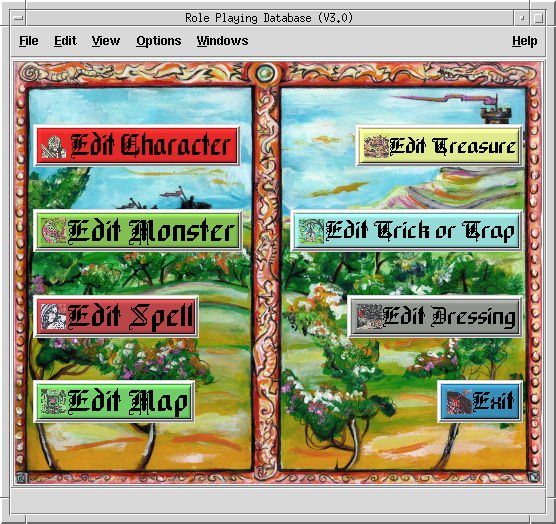
\includegraphics[width=5in]{MainWindow.png}
\caption{The main window of the Role Playing Database}
\label{fig:main}
\end{centering}
\end{figure}

\section{Sheet Template Editor Window}
\label{Template}

\begin{figure}[hbpt]
\begin{centering}
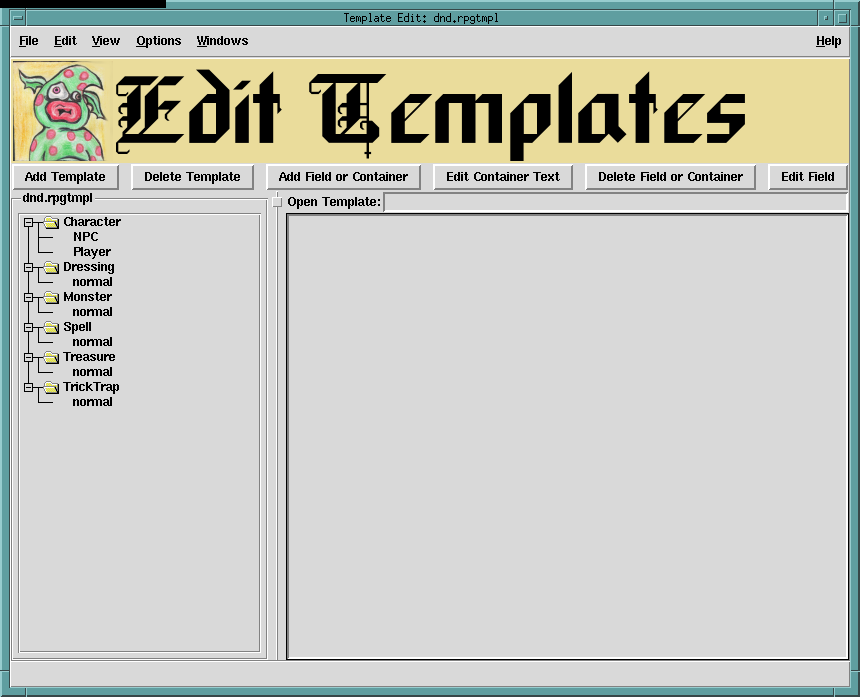
\includegraphics[width=5in]{TemplateEditor1.png}
\caption{The initial Template Editor Window}
\label{fig:tmped1}
\end{centering}
\end{figure}

\begin{figure}[hbpt]
\begin{centering}
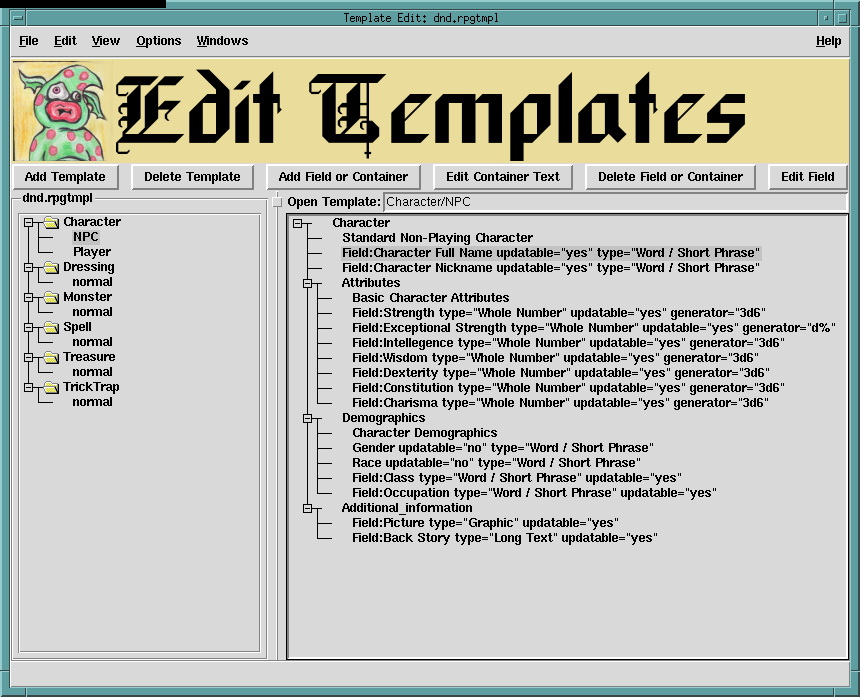
\includegraphics[width=5in]{TemplateEditor2.png}
\caption{The Template Editor Window after loading a template}
\label{fig:tmped2}
\end{centering}
\end{figure}

\section{Character Editing Window}
\label{Character}

\begin{figure}[hbpt]
\begin{centering}
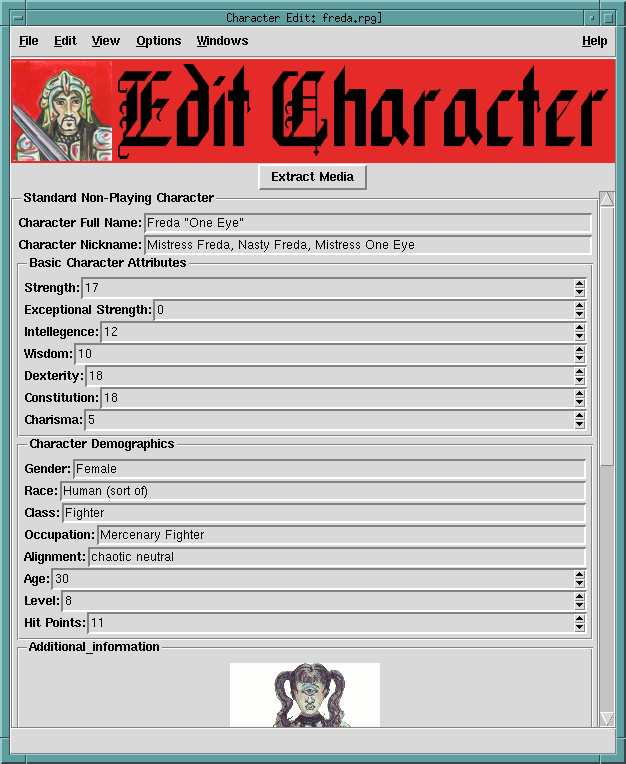
\includegraphics[width=5in]{CharacterEditor.png}
\caption{The Character Editor window of the Role Playing Database}
\label{fig:char}
\end{centering}
\end{figure}

\section{Monster Editing Window}
\label{Monster}

\section{Spell Editing Window}
\label{Spell}

\section{Treasure Editing Window}
\label{Treasure}

\section{Trick / Trap Editing Window}
\label{TrickTrap}

\section{Dressing Editing Window}
\label{Dressing}

\section{Map Editing Window}
\label{Map}


